\documentclass[a4paper, 10pt, dvipdfmx]{jlreq}

\usepackage{amsmath,amsfonts,amssymb}
\usepackage{bm}
\usepackage{mathtools}
\usepackage{siunitx}
\usepackage[dvipdfmx]{graphicx}
\usepackage[dvipdfmx]{color}
\usepackage[dvipdfmx, colorlinks=true, allcolors=blue]{hyperref}
\usepackage{listings}
\usepackage{tikz}
\usepackage{physics}
\usepackage{url}

\Urlmuskip=0mu plus 10mu
\allowdisplaybreaks[4]
\frenchspacing
\definecolor{OliveGreen}{rgb}{0.0,0.6,0.0}
\definecolor{Orange}{rgb}{0.89,0.55,0}
\definecolor{SkyBlue}{rgb}{0.28, 0.28, 0.95}
\lstset{
  language={c++},
  basicstyle={\ttfamily},
  identifierstyle={\small},
  ndkeywordstyle={\small},
  frame=single,
  breaklines=true,
  numbers=left,
  xrightmargin=0zw,
  xleftmargin=3zw,
  numberstyle={\scriptsize},
  lineskip=-0.9ex,
  keywordstyle={\small\bfseries\color{SkyBlue}},  
  commentstyle={\color{OliveGreen}}, 
  stringstyle={\small\ttfamily\color{Orange}}    
}

\begin{document}

\title{2015年度 大問4}
\author{hari64boli64 (hari64boli64@gmail.com)}
\date{\today}
\maketitle

\section{問題}

$I=[0,1],I_1=[0,\frac{1}{2}],I_2=[\frac{1}{2},1]$

\begin{align*}
  f(x)=\begin{cases}
         x+\frac{1}{2} & (x\in I_1)  \\
         2-2x          & (x \in I_2)
       \end{cases}
\end{align*}

\section{解答}

\begin{figure}[htbp]
  \begin{center}
    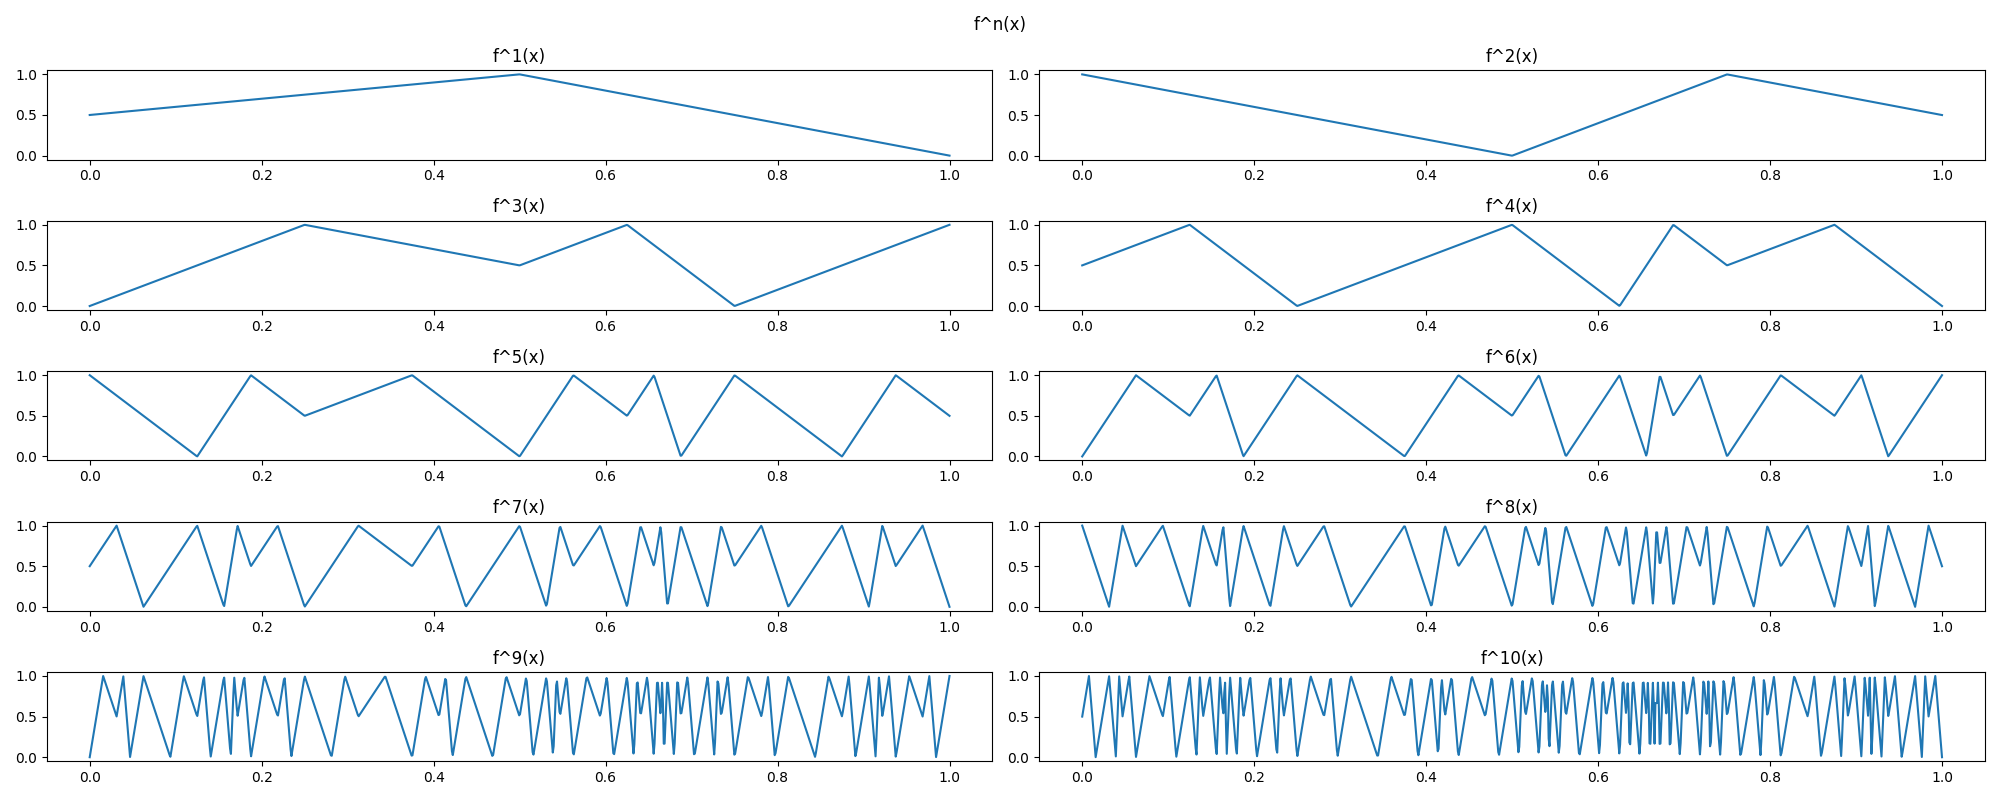
\includegraphics[width=140mm]{4.png}
    \caption{$f^n(x)$}
    \label{img:fnx}
  \end{center}
\end{figure}

\subsection*{(1)}

$J$は閉区間であって、閉集合ではないことに注意。

この点さえ分かっていれば、中間値の定理より自明。

\subsection*{(2)}

\subsubsection*{(2-1)}

不明

\subsubsection*{(2-2)}

自明

\subsubsection*{(2-3)}

存在性は不明。

一意性は(2-2)より自明。

\subsection*{(3)}

隣接行列の意味より自明。(大嘘)

\subsection*{(4)}

対角化して求めればよい。(todo)

実は、フィボナッチ数列が出てくる。(おまけ参照)

よって、ビネの公式より、求める値は$\frac{1+\sqrt{5}}{2}$となる。

\section{知識}

ビネの公式は、以下の通り。\cite{site:binet}

\begin{equation*}
  F_n=\frac{1}{\sqrt{5}}\left\{ \left( \frac{1+\sqrt{5}}{2} \right)^n - \left( \frac{1-\sqrt{5}}{2} \right)^n \right\}
\end{equation*}

\section{おまけ}

\lstinputlisting[caption=calculateLimit,label=code:calculateLimit,language=Python]{4.py}

\begin{lstlisting}[caption=result, label=code:result]
n: 1, A^n: [[0, 1], [1, 1]]
trace: 1
n: 2, A^n: [[1, 1], [1, 2]]
trace: 3
n: 3, A^n: [[1, 2], [2, 3]]
trace: 4
n: 4, A^n: [[2, 3], [3, 5]]
trace: 7
n: 5, A^n: [[3, 5], [5, 8]]
trace: 11
n: 6, A^n: [[5, 8], [8, 13]]
trace: 18
n: 7, A^n: [[8, 13], [13, 21]]
trace: 29
n: 8, A^n: [[13, 21], [21, 34]]
trace: 47
n: 9, A^n: [[21, 34], [34, 55]]
trace: 76
==========
limit of logN(p)/p:  0.4812118250596034
math.log((1+math.sqrt(5))/2)=0.48121182505960347
\end{lstlisting}

\begin{thebibliography}{9}
  \bibitem{site:binet}
  高校数学の美しい物語.``フィボナッチ数列の7つの性質(一般項・黄金比・互いに素)''.2021年8月17日.\url{https://manabitimes.jp/math/643}
\end{thebibliography}

\end{document}
